\documentclass[12pt,letterpaper]{article}
\usepackage[utf8]{inputenc}

\usepackage{graphicx}
\setlength{\parskip}{0.4em}
\setlength{\parindent}{0em}

\begin{document}
\title{

\includegraphics[width=0.3\textwidth]{National_Institute_of_Technology,_Raipur_Logo.png}
\\ 
Hidden Markov Model (HMM)
}

\author{SHREEDUTT 19111056 BME 5TH SEMESTER}

\maketitle
\rule{\textwidth}{0.5pt}
\\
\subsection*{Introduction}
\textbf{Hidden Markov Model (HMM)} is a statistical Markov model in which the system being modeled is assumed to be a Markov process with unobserved (i.e. hidden) states.
\\
Hidden Markov models are especially known for their application in reinforcement learning and temporal pattern recognition such as speech, handwriting, gesture recognition, part-of-speech tagging, musical score following, partial discharges and bioinformatics.
\\
Biological sequence analysis is frequently as simple as affixing the appropriate label to each residue. We want to label nucleotides as exons, introns, or intergenic sequences in gene identification. We want to associate residues in a query sequence with homologous residues in a target database sequence in sequence alignment. 
\\
\\
\subsubsection*{Terminology in HMM}
For example, the term "hidden" refers to the first-order Markov process that lies behind the observation in question. An observation is any data that we are aware of or that we can observe. These HIDDEN STATES can be seen in the following diagram, where "Rainy" interacts with "Sunny".
\\
\\
\begin{figure}[htp]
    \centering
    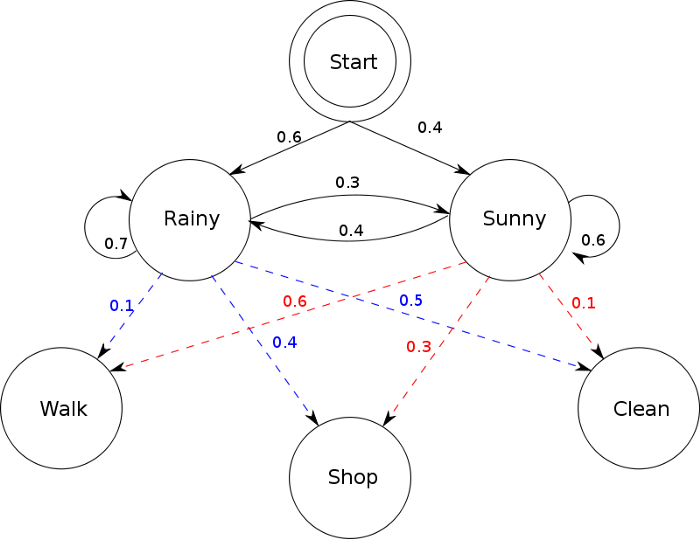
\includegraphics[width=.95\textwidth]{Hmm.png}
\end{figure}
\\
\\
As shown in the diagram, OBSERVATIONS refers to the words "Walk", "Shop", and "Clean". Our observations are our training data in machine learning, and the number of hidden states is our hyper parameter for our model. The model's evaluation will be discussed in a future post.
\\
\\
\textbf{T} = length of the observation sequence
\\
\textbf{N} = number of states in the model 
\\
\textbf{M} = number of observation symbols
\\
\textbf{Q} = \{ \[q_0,q_1,.... ,q_{N - 1}\] \} = distinct states of the Markov process
\\
\textbf{V} = \{ 0, 1, ..... , M - 1\} = set of possible observations
\\
\textbf{A} = state transition probabilities
\\
\textbf{B} = observation probability matrix
\\
\textbf{$\Pi$} = initial state distribution
\\
\textbf{O} = ( \[O_0, O_1, ...., O_{T - 1}\] ) = observation sequence.
\\
\\
T = don’t have any observation yet,
\\
N = 2,
\\
M = 3,
\\
Q = \{``Rainy”, ``Sunny”\},
\\
V = \{``Walk”, ``Shop”, ``Clean”\}
\\
\\
Each hidden state's transition probabilities are represented by arrows. The blue and red arrows point to each observation from each hidden state in the observation probability matrix. A row stochastic matrix means that the rows add up to one in each matrix row.
\[ a_{ij} = P(state q_j at t + 1 |  state q_i at t) \]
\[ b_j(k) = P(observation k at | state q_j at t) \]
\\ 
This is a full model with known state transition probabilities.
\\ 
\[\lambda = (A, B, \pi) \]



\end{document}







